Durant notre première séance de laboratoire pour le cours de physique des télécommunications, nous avons dimensionné notre antenne patch à l'aide du logiciel FEKO. Pour cela nous avons procédé par étapes, partant d'un design extrêmement simple auquel nous avons petit à petit ajouté ou modifié des éléments pour arriver à la version finale de notre antenne.
A la fin de la séance, notre antenne avait un coefficient de réflexion minimal de \SI{-27.43}{\deci\bel} à la fréquence de \SI{2.398}{\giga\hertz} là où le cahier des charges nous imposait un coefficient de réflexion de \SI{-6}{\deci\bel} à la fréquence d'utilisation de l'antenne, c'est-à-dire \SI{2.4}{\giga\hertz}.

Dans ce chapitre, nous allons détailler les différentes étapes qui nous ont amené au dimensionnement final de notre antenne.


\subsection{Antenne sur un diélectrique infini}
Pour commencer, nous avons simplement simulé un patch rectangulaire posé sur un matériau diélectrique de même permittivité électrique que le PCB utilisé en pratique pour fabriquer notre antenne. Pour ce qui est des dimensions (longueur et largeur) du patch, nous avons utilisé les formules qui nous étaient fournies. La figure \ref{fig:rayonnement_11} nous donne la directivité ainsi que le gain de l'antenne pour des valeurs de $\phi$ de \SI{0}{\degree} et \SI{90}{\degree}.
\begin{figure}[htbp]
  \centering
  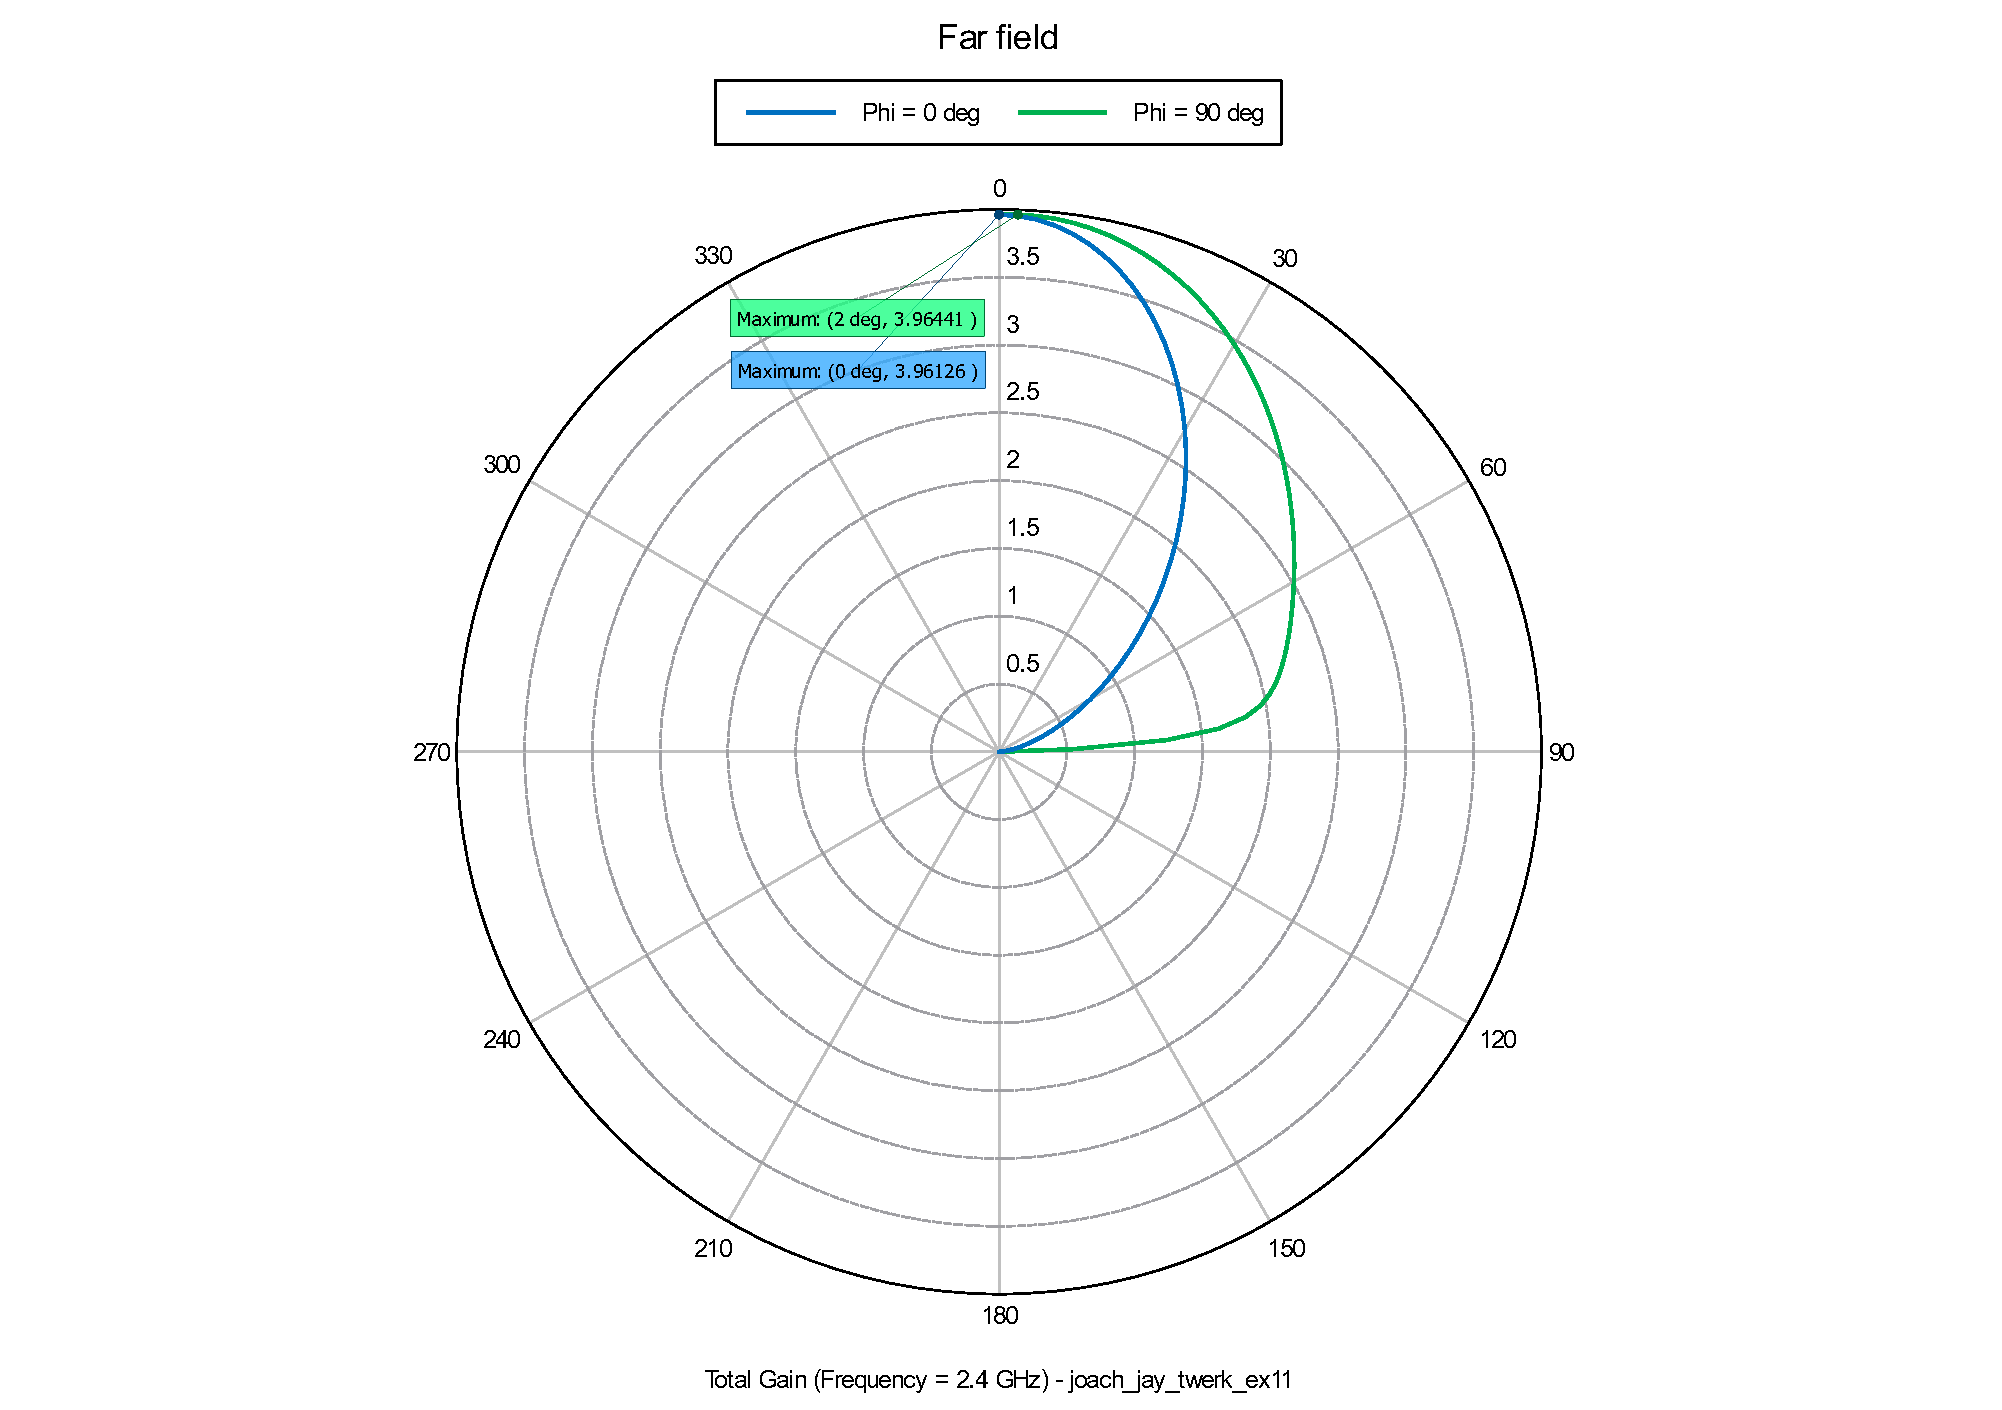
\includegraphics[width=0.7\textwidth]{rayonnement11_annotation.pdf}
  \caption{Diagramme de rayonnement du gain [généré avec PostFeko]\label{fig:rayonnement_11}}
\end{figure}
Pour les deux valeurs de $\phi$, la directivité maximale est de \SI{0}{\degree}.

Nous nous sommes aussi intéressés au coefficient de réflexion de l'antenne ainsi qu'à sa fréquence de résonance.
\begin{figure}[htbp]
  \centering
  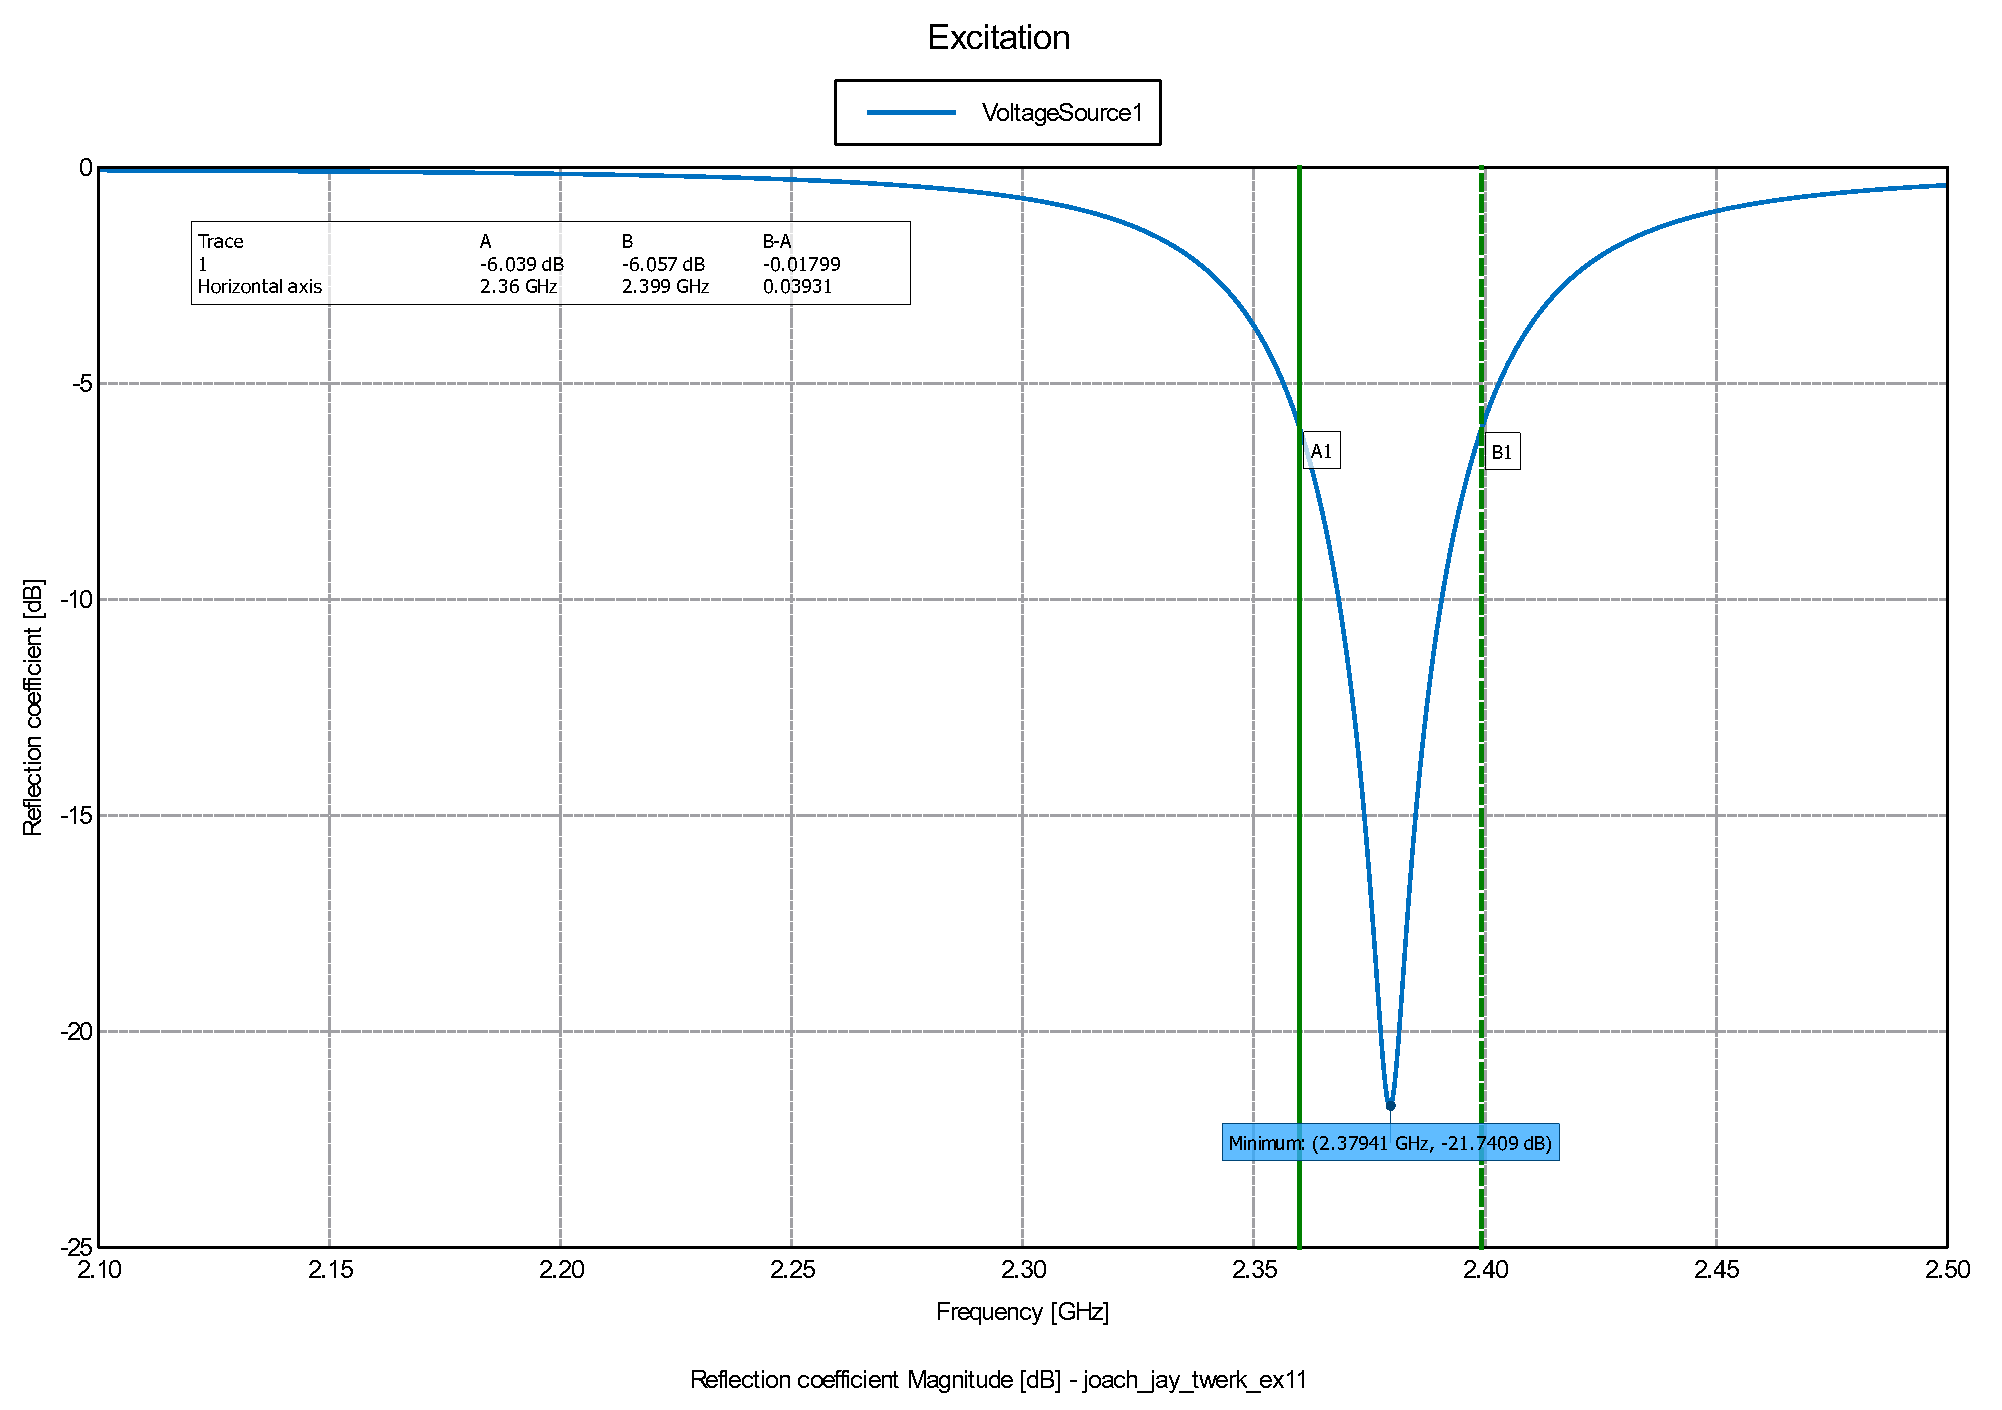
\includegraphics[width=0.7\textwidth]{reflection11_annotation.pdf}
  \caption{Coefficient de réflexion en fonction de la fréquence [généré avec PostFeko]\label{fig:reflection11_}}
\end{figure}
La figure \ref{fig:reflection11_} nous montre que la résonance de l'antenne se situe à \SI{2.37941}{\giga\hertz} qu'à cette fréquence le coefficient de réflexion vaut \SI{-21.8}{\deci\bel}. A \SI{2.4}{\giga\hertz} ce coefficient vaut \SI{-6}{\deci\bel}, il est intéressant de noter la valeur de la bande passante définie à \SI{-6}{\deci\bel} qui vaut ici pas loin de \SI{0.04}{\giga\hertz}. Un dernier aspect important pour ce point est le pourcentage de puissance délivrée à l'antenne à la fois à la fréquence de résonance et à \SI{2.4}{\giga\hertz}. Ce pourcentage nous est donné par la formule \ref{eqn:puissance délivrée}, ce qui nous donne une valeur de \SI{84}{\percent} à la fréquence de résonance et \SI{25}{\percent} à \SI{2.4}{\giga\hertz}.
\begin{equation}
P = {(1-\Gamma_L)^2}
\label{eqn:puissance délivrée}
\end{equation}

%Note pour jojol: coeff de réflection c'est gamma majuscule, aka \Gamma_L (L pour load).
%Merci d'utiliser \SI! c'est vachement cool!
%Je me suis planté, la proportion absorbée c'est 1-(gamma)². Je m'occupe (ou me suis occupé) de corriger dans ce qui est déjà fait.
